\chapter{Экспериментальная часть}

В данном разделе описаны замерные эксперименты и представлены результаты исследования.

\section{Технические характеристики}
Технические характеристики устройства, на котором выполнялся эксперимент \cite{bib:5}:
\begin{itemize}
	\item 8 ГБ оперативной памяти;
	\item процессор Apple M2 (тактовая частота~---~до $3.5$ГГц);
    \item операционная система macOS Ventura 13.0.
\end{itemize}

\section{Измерение процессорного времени выполнения реализаций алгоритмов}

Для измерения процессорного времени выполнения реализаций алгоритмов была использована функция языка $C$~---~$clock\_gettime$, которая позволяет получить текущее процессорное время в наносекундах \cite{bib:6}.

\subsection{Худший случай}

В таблице \ref{table:time_worst} представлены результаты измерений процессорного времени выполнения в зависимости от размерности квадратной матрицы для худшего случая алгоритма Винограда. На рисунке \ref{img:time_worst} представлена зависимость времени выполнения от размерности квадратной матрицы.

\begin{table}[h]
  \caption{\label{table:time_worst} Результаты замеров процессорного времени для худшего случая (в нс)}
  \begin{center}
    \begin{tabular}{|r|r|r|r|}
      \hline
      Размерность & Обычный & Виноград & Опт. Виноград\\ \hline
      1 & 241 & 472 & 442 \\ \hline
      3 & 330 & 559 & 418 \\ \hline
      5 & 544 & 637 & 582 \\ \hline
      7 & 840 & 876 & 768 \\ \hline
      9 & 1291 & 1231 & 1073 \\ \hline
      13 & 3551 & 2898 & 2626 \\ \hline
      15 & 5585 & 4230 & 3891 \\ \hline
      19 & 11254 & 7824 & 7268 \\ \hline
      29 & 41766 & 27095 & 24959 \\ \hline
      39 & 108670 & 62862 & 60685 \\ \hline
      49 & 231702 & 123522 & 120280 \\ \hline
      59 & 427248 & 218014 & 226923 \\ \hline
    \end{tabular}
  \end{center}
\end{table}

\newpage

\noindent
\begin{figure}[h!]
	\centering
    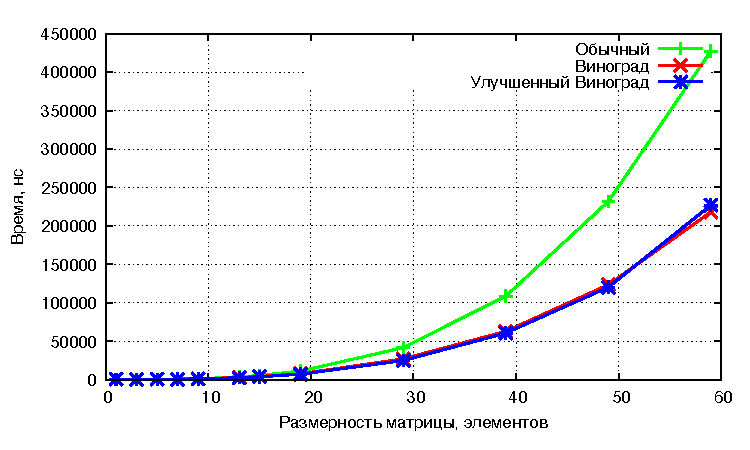
\includegraphics[width=0.75\linewidth]{../data/time_worst}
    \caption{Результаты замеров времени для худшего случая}
    \label{img:time_worst}
\end{figure}

Так как на этом масштабе не видна разница между реализациями алгоритма Винограда и оптимизированного алгоритма Винограда, то на рисунке \ref{img:time_winograd_worst} представлена зависимость времени выполнения от размерности квадратной матрицы для данных двух алгоритмов на более показательном масштабе.

\noindent
\begin{figure}[h!]
	\centering
    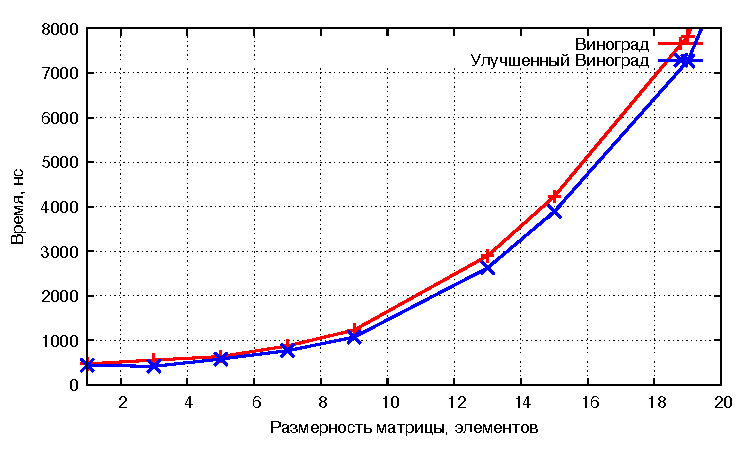
\includegraphics[width=0.75\linewidth]{../data/time_winograd_worst}
    \caption{Результаты замеров времени для алгоритма Винограда и его оптимизированного варианта}
    \label{img:time_winograd_worst}
\end{figure}


\subsection{Лучший случай}

В таблице \ref{table:time_best} представлены результаты измерений процессорного времени выполнения в зависимости от размерности квадратной матрицы для худшего случая алгоритма Винограда. На рисунке \ref{img:time_best} представлена зависимость времени выполнения от размерности квадратной матрицы.

\begin{table}[h]
  \caption{\label{table:time_best} Результаты замеров процессорного времени для лучшего случая (в нс)}
  \begin{center}
    \begin{tabular}{|r|r|r|r|}
      \hline
      Размерность & Обычный & Виноград & Опт. Виноград\\ \hline
      2 & 389 & 579 & 494 \\ \hline
      4 & 548 & 588 & 501 \\ \hline
      6 & 739 & 737 & 680 \\ \hline
      8 & 1074 & 1014 & 920 \\ \hline
      10 & 1074 & 1440 & 1337 \\ \hline
      14 & 4405 & 3397 & 3113 \\ \hline
      16 & 6783 & 4890 & 4508 \\ \hline
      20 & 13310 & 9288 & 8213 \\ \hline
      30 & 48497 & 31234 & 33992 \\ \hline
      40 & 121926 & 67162 & 64612 \\ \hline
      50 & 255559 & 132789 & 132273 \\ \hline
      60 & 453096 & 228107 & 225757 \\ \hline
    \end{tabular}
  \end{center}
\end{table}

\newpage

\noindent
\begin{figure}[h!]
	\centering
    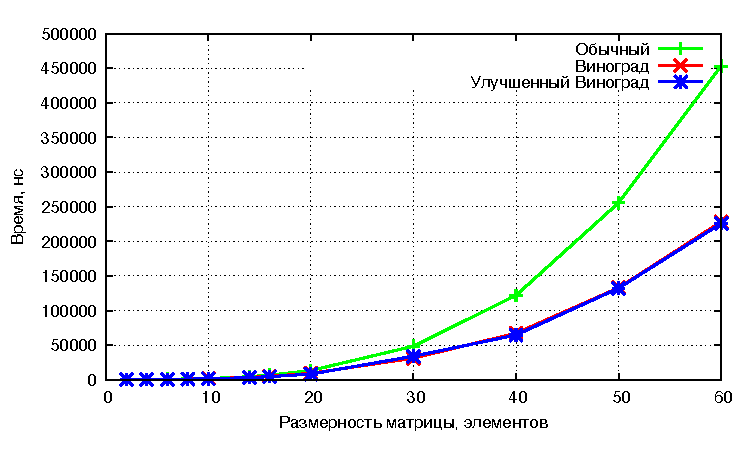
\includegraphics[width=0.75\linewidth]{../data/time_best}
    \caption{Результаты замеров времени для лучшего случая}
    \label{img:time_best}
\end{figure}

Так как на этом масштабе не видна разница между реализациями алгоритма Винограда и оптимизированного алгоритма Винограда, то на рисунке \ref{img:time_winograd_best} представлена зависимость времени выполнения от размерности квадратной матрицы для данных двух алгоритмов на более показательном масштабе.

\noindent
\begin{figure}[h!]
	\centering
    \includegraphics[width=0.75\linewidth]{../data/time_winograd_best}
    \caption{Результаты замеров времени для алгоритма Винограда и его оптимизированного варианта}
    \label{img:time_winograd_best}
\end{figure}


\section{Измерение объёма потребляемой памяти реализаций алгоритмов}

В таблице \ref{table:memory} представлены результаты измерения потребляемой памяти в зависимости от размерности квадратной матрицы. На рисунке \ref{img:memory} представлена зависимость потребляемой памяти от размерности квадратной матрицы.

\begin{table}[h]
  \caption{\label{table:memory} Результаты замеров потребляемой памяти (в байтах)}
  \begin{center}
    \begin{tabular}{|r|r|r|r|}
      \hline
      Размерность & Обычный & Виноград & Опт. Виноград\\ \hline
      1 & 176 & 336 & 353 \\ \hline
      2 & 224 & 392 & 409 \\ \hline
      3 & 288 & 464 & 481 \\ \hline
      4 & 368 & 552 & 569 \\ \hline
      5 & 464 & 656 & 673 \\ \hline
      6 & 576 & 776 & 793 \\ \hline
      7 & 704 & 912 & 929 \\ \hline
      8 & 848 & 1064 & 1081 \\ \hline
      10 & 1184 & 1416 & 1433 \\ \hline
      13 & 1808 & 2064 & 2081 \\ \hline
      16 & 2576 & 2856 & 2873 \\ \hline
      20 & 3824 & 4136 & 4153 \\ \hline
      30 & 8064 & 8456 & 8473 \\ \hline
      40 & 13904 & 14376 & 14393 \\ \hline
      50 & 21344 & 21896 & 21913 \\ \hline
      60 & 30384 & 31016 & 31033 \\ \hline
    \end{tabular}
  \end{center}
\end{table}

\newpage

\noindent
\begin{figure}[h!]
	\centering
    \includegraphics[width=0.75\linewidth]{../data/memory.pdf}
    \caption{Результаты замеров памяти}
    \label{img:memory}
\end{figure}

Так как на этом масштабе не видна разница между реализациями алгоритмов, то на рисунке \ref{img:memory_detail} представлена зависимость потребляемой памяти от размерности квадратной матрицы на более показательном масштабе.

\noindent
\begin{figure}[h!]
	\centering
    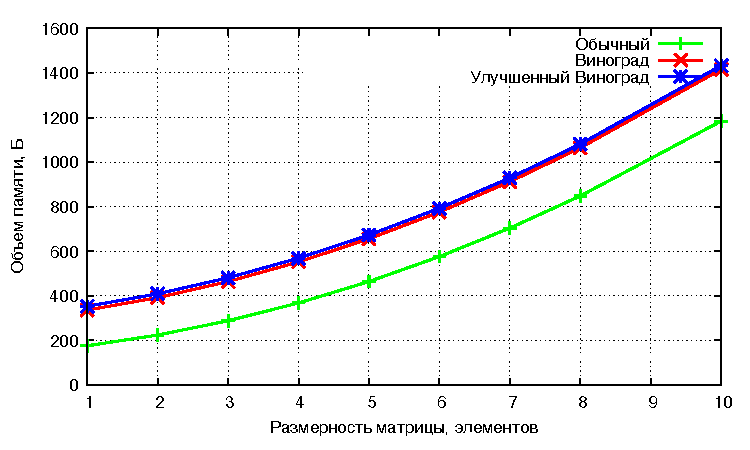
\includegraphics[width=0.75\linewidth]{../data/memory_detail.pdf}
    \caption{Результаты замеров памяти (увеличенный масштаб)}
    \label{img:memory_detail}
\end{figure}

\newpage